%  Created by Etienne van Delden on 2010-03-03.
%  Copyright (c) 2010 TU/e & Anson, Edin, Etienne. All rights reserved.
%
\documentclass[a4paper]{article}

% Use utf-8 encoding for foreign characters
\usepackage[utf8]{inputenc}

% Setup for fullpage use
%\usepackage{fullpage}

% Uncomment some of the following if you use the features
%
% Running Headers and footers
\usepackage{fancyhdr}

% Use colored links
\usepackage[pdftex,colorlinks]{hyperref}

% Multipart figures
%\usepackage{subfigure}

% More symbols
\usepackage{amsmath}
\usepackage{amssymb}
\usepackage{latexsym}

% Surround parts of graphics with box
\usepackage{boxedminipage}

% Package for including code in the document
\usepackage{listings}

% If you want to generate a toc for each chapter (use with book)
\usepackage{minitoc}

% This is now the recommended way for checking for PDFLaTeX:
\usepackage{ifpdf}

%\newif\ifpdf
%\ifx\pdfoutput\undefined
%\pdffalse % we are not running PDFLaTeX
%\else
%\pdfoutput=1 % we are running PDFLaTeX
%\pdftrue
%\fi

\ifpdf
\usepackage[pdftex]{graphicx}
\else
\usepackage{graphicx}
\fi
\title{A student/teach collaboration web application}
\author{}

\date{2010-03-03}

\begin{document}

\ifpdf
\DeclareGraphicsExtensions{.pdf, .jpg, .tif}
\else
\DeclareGraphicsExtensions{.eps, .jpg}
\fi

\maketitle


\begin{abstract}
  Our idea for a collaboration web application, targeted to both students and teachers.
\end{abstract}



\section{The web application} % (fold) (oh? leid eens af, dan! ik zie geen smiley :P)
\label{sec:web-app}
    Our project is an education cooperation website. The two main purposes will be aiding students and teachers in
\begin{enumerate}
	\item learning about (technical) topics of their interest
	\item organizing, and taking part in, courses
 \end{enumerate}
  The two mechanisms for this will be
\begin{enumerate}
	 \item[a] sharing information and,
	 \item[b] finding people with the same interests/courses or with required expertise/position (for ex. possible tutors or instructors).
\end{enumerate}

 \begin{description}
      \item[What this project is:] Our web-app will occupy a place between Wikipedia-like information sources and social or professional networking sites; it enables sharing information and helps education, but not anonymously or in one specific format, and it facilitates networking and cooperation, but always with a focus on creating/improving documents and furthering one's education.
      \item[What this project is not:] This app is not intended to be a complete portal, like Studyweb or Sakai, nor to be as hierarchically organized. It's not an official information source like OWinfo or TUe.nl. It's not an evaluation or validation system like Peach, a place to share unfinished, internal work like a Subversion server, a project management system like Projexy, or an email client like Outlook.
      \item[Features:]
       \begin{enumerate}
                       \item Must-have features: Personal accounts, an RDF database of objects (``documents''), some standard types/topics.
                       \item Should-have features: Personal pages, RSS feeds, egalitarian organization, commenting on documents, dynamic output.
                       \item Could-have features: An elaborate branching/updating/approval/authorship (not ``ownership''!) system, ``following'' people %redundant => RSS feeds ?
                       \item Would-have features: API, links to (external) email accounts, licensing notice support, user-controlled type merging
                     \end{enumerate}
      \item[Searching:]Ideally one could search the database by adding or subtracting categories in any order. For example: a user should be able to search by choosing everything related only to the course Databases, then, from among the results, choosing all documents of type summaries, and then, from the results of that, choosing everything authored or co-authored by person A, then see only old versions. The user should be able to find the same thing by first choosing ``author: contains A'', then ``type: only summaries'', then ``versions: not current'', and then ``course: only Databases''.
    \end{description}
% section The web application (end)

\section{Tools}
\begin{itemize} % Justification for each tool? Lijst tools op http://wwwis.win.tue.nl/~webtechnologie/2II25/assign.html gecheckt?
                % Wat moet er dan van justification erbij? We denken dat we hiermee aan de slag mee kunnen, en verder niets. Echte redenen waarom we perse dit willen gebruiken weet ik niet. Misschien omdat dat genoemd is op de slides en website?
  \item Our web pages will be built by using \emph{HTML} for the general structure, \emph{CSS} for the layout and \emph{Javascript/AJAX} for dynamic interaction.
  \item For our rdf storage we will use \emph{Redland} and for the queries \emph{SPARQL}. The choice for \emph{Redland} is because of the recommendation in the book, but also because of the support for \emph{RSS} and \emph{Atom} feeds which are a "should have" on our priority list.
  \item The web application will be built in \emph{Python} by using the HTTP framework \emph{CherryPy}~\cite{cherrypy}. % alternatieven: twisted, django
  \item For our web pages we will also use \emph{Mako Templates}~\cite{mako}.
\end{itemize}
% section Tools (end)

\section{Discussion} % (fold)
\label{sec:discussion}
  % Check LaTeX image auto-placement.
  For our database we have two demands:

  \begin{itemize}
    \item We want to store a lot of content
    \item It needs to be expandable in a modular fashion
  \end{itemize}

What kind of content do we want to add? While investigating this, we stumbled upon a realization. The content we want to store is of a different kind for different groups of people. While teachers are only interested in serving \emph{courses}, \emph{course information} and \emph{lectures}, students are interested in \emph{summaries}, \emph{discussions} and study tools. The italic words are the different types of content that may or may not be used in our web-app. But they all have a common structure: they have a name, the content itself and a certain type.  We have visualized this general structure in Figure~\ref{fig:structure}.\\
\\
For example, a student could make a summary (the type), called ``Summary - 2II25'' for the course ``Web Technology'' (the name of a related course) with a piece of text explaining a number of topics (a blank node, with relations to other content). Such a topic could be RDF (the name), which is a topic (the type) and has text with the actual information for the user.\\
\\
A teacher would be interested in different content. He could add a course (a type) called ``Web Technology'' (the name) with some content. This content could be course information (both name and type) with text explaining what the course is about. It could also have a lectures page (again both name and type) with lecture slides (some files).\\
\\
Visually, these examples are shown in respectively Figure~\ref{fig:exstudent} and Figure~\ref{fig:exteacher}, and combined in Figure~\ref{fig:combined}.
\\

\begin{figure}[!htb]
	\centering
	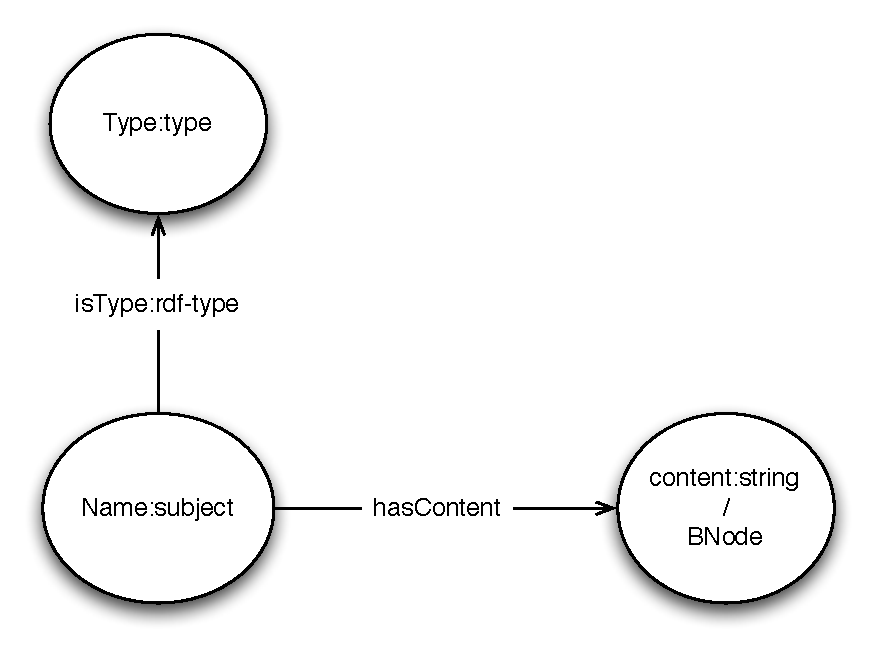
\includegraphics[scale=0.5]{photos/structure}
	\caption{The structure of content}
	\label{fig:structure}
\end{figure}

\begin{figure}[!htb]
	\centering
	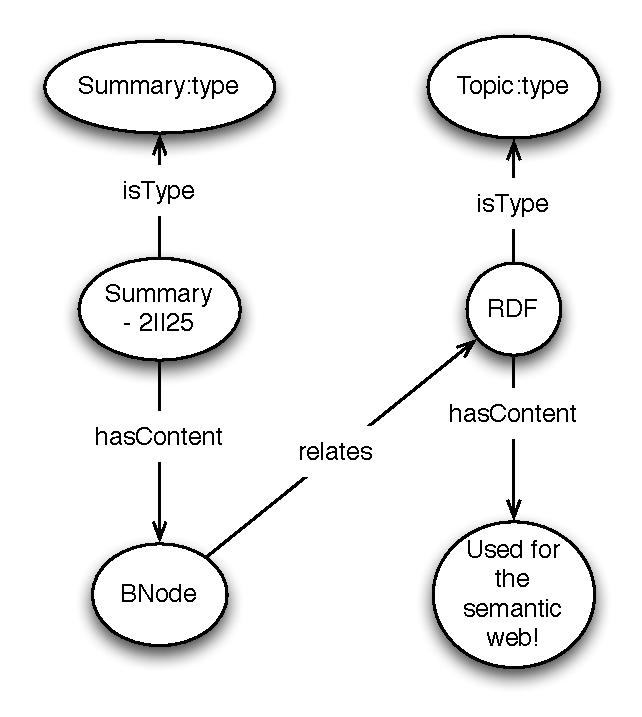
\includegraphics[scale=0.5]{photos/exstudent}
	\caption{An example of content a student would add}
	\label{fig:exstudent}
\end{figure}

\begin{figure}[!htb]
	\centering
	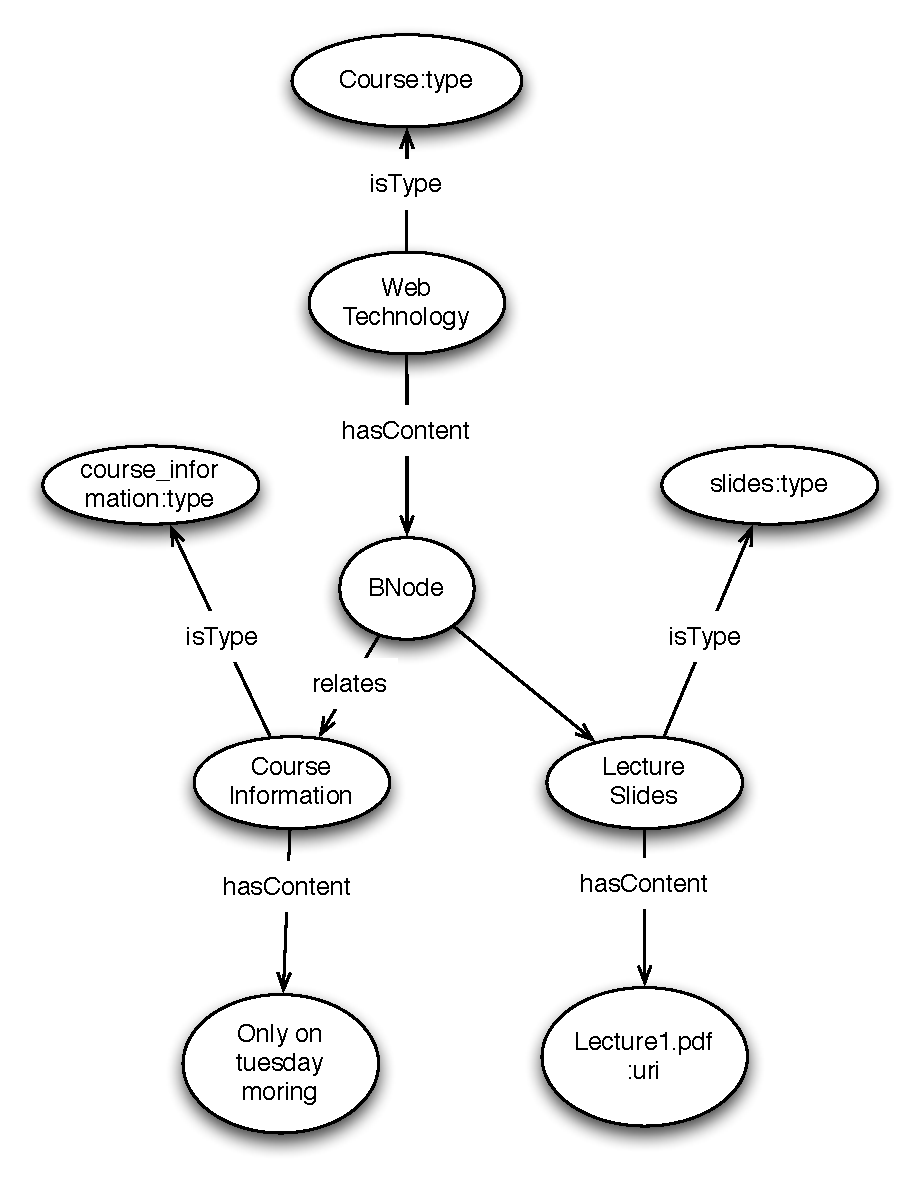
\includegraphics[scale=0.5]{photos/exteacher}
	\caption{An example of the content a teacher would add}
	\label{fig:exteacher}
\end{figure}

\begin{figure}[!ht]
	\centering
	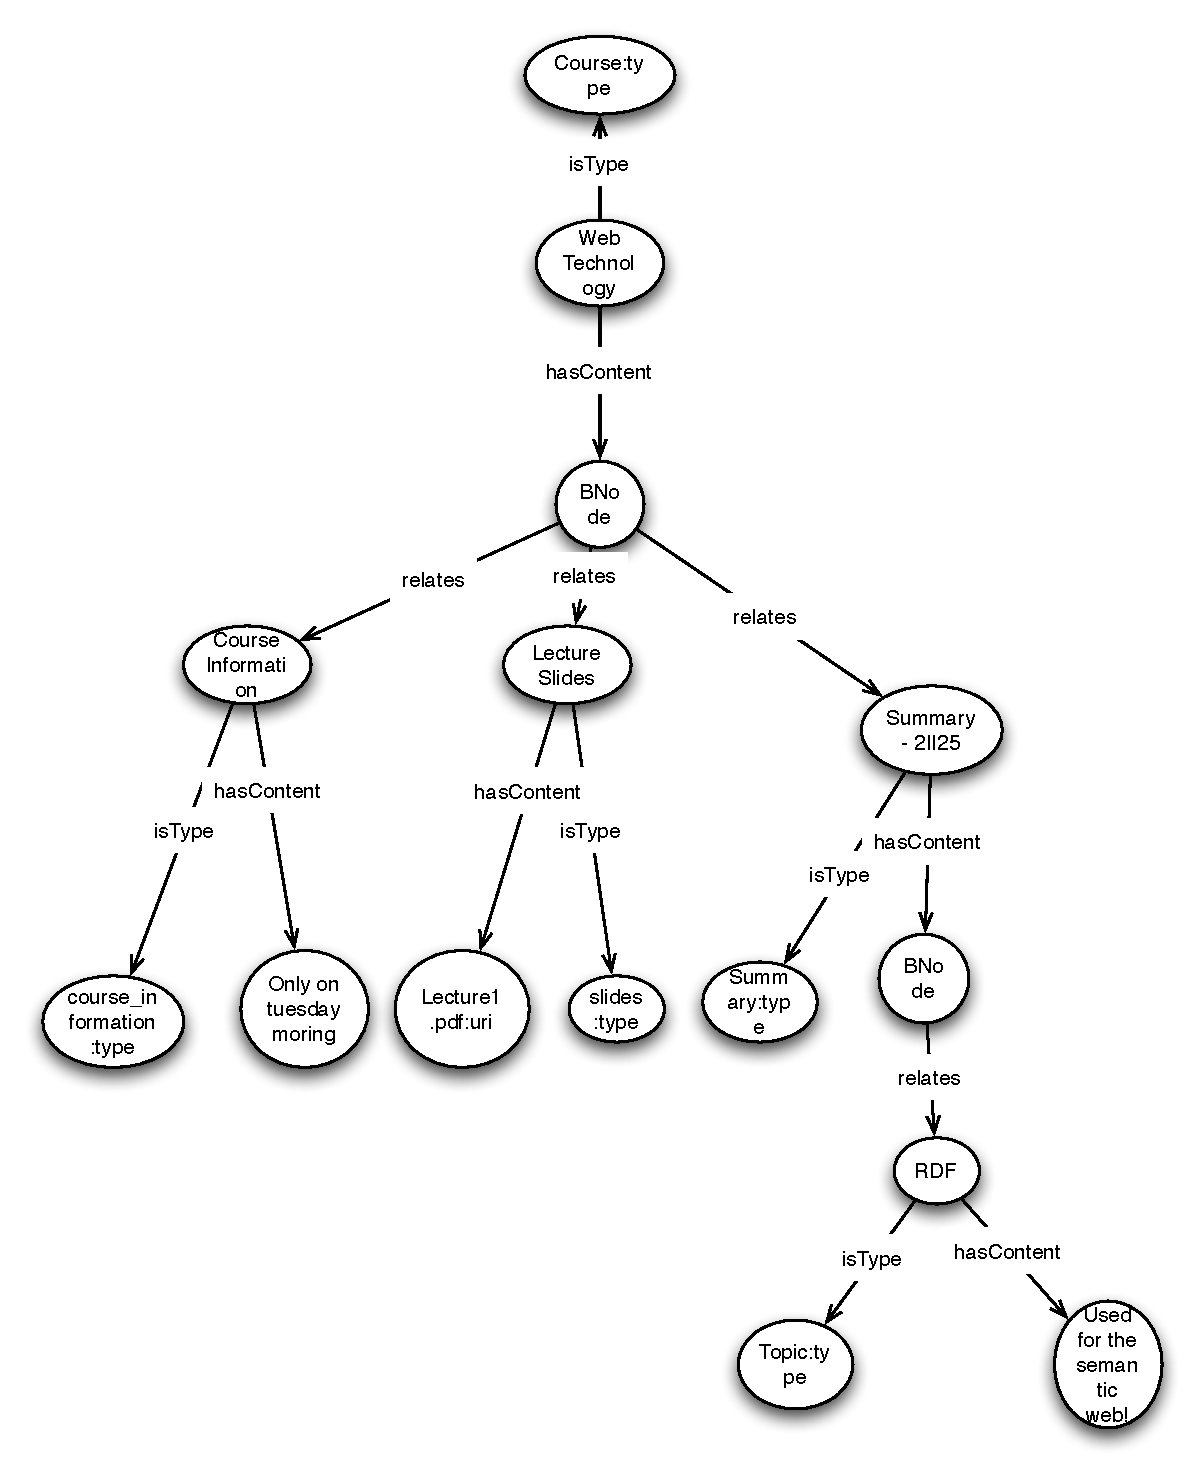
\includegraphics[width=11cm,height=14cm]{photos/combined}
	\caption{The RDF database, both examples combined}
	\label{fig:combined}
\end{figure}

Users can easily add their own content by relating it to an existing type. Users can also easily search by document type. Depending on how much we can implement in the given time, we can also assign properties to documents of a certain type. We could, for example, make it a property that a piece of content of a certain type may not have sub-content, only text, or the contrary; that it can only have other content. Using the current model, we can just add a property to a type, and all documents of that type will then have been changed.\\
\\
We also abstract from giving objects pre-defined types. A Dutch localization of our web-app could easily use the type ``samenvatting'', instead of ``summary''. But, even more powerful: the users can determine what kind of content they add. A summary, paragraph, question, course information, topic discussion, anything meaningful to the users can be added. We could somehow ``merge'' types which are essentially the same (such as ``samenvatting'' and ``summary''), while remembering its different names.\\
\\
Ownership can also be easily expressed in an RDF model. When ever new content is made, a relationship with the creator is made, making him the owner. Then, when someone creates a new ``branch'' of the object, the original creator can ``approve'' it, to label it as an updated version of the older object. This will help us to create the social networking aspect of our web-app. When someone ``follows'' a person, we could easily  find  all content created by a person and show the changed content. \\
\\
RDF is a really powerful data-model to express relationships. By using RDF, we can relate all kinds of different data, and easily add new features by simple creating a new relationship. This makes RDF the perfect solution for our needs.
% section Discussion (end)



\bibliographystyle{plain}
\begin{thebibliography}{}
\bibitem{cherrypy}
  http://www.cherrypy.org/
\bibitem{mako}
  http://www.makotemplates.org/
\end{thebibliography}

\end{document} 